\documentclass[10pt,twocolumn,letterpaper]{article}
\usepackage[T1]{fontenc}
\usepackage[review]{cvpr}
\usepackage{amsmath,amssymb,graphicx,booktabs,multirow}
\definecolor{cvprblue}{rgb}{0.21,0.49,0.74}
\usepackage[pagebackref,breaklinks,colorlinks,allcolors=cvprblue]{hyperref}
\def\paperID{*****}
\def\confName{CVPR}
\def\confYear{2027}
\newcommand{\method}{DecisionICL\xspace}
\newcommand{\train}{\mathcal{T}}
\newcommand{\valid}{\mathcal{V}}
\newcommand{\classes}{\mathcal{C}}
\newcommand{\argmax}{\operatorname*{arg\,max}}
\newcommand{\TopK}{\operatorname{TopK}}
\newcommand{\JSD}{\operatorname{JSD}}
\title{DecisionICL\\Selecting Visual Demonstrations with Target-Model Decision Factors}
\author{Anonymous authors}
\begin{document}
\maketitle

\begin{abstract}
Visual in-context learning uses labeled demonstrations in a vision-language model's prompt to classify a query. With one or two demonstrations, retrieval must convey useful visual distinctions. We introduce \method to guide retrieval with decision factors elicited from the target model. Each factor describes a visual property and its possible states. A frozen image-text encoder measures these states. Labeled training images define class prototypes in the resulting factor space. Class selection maximizes a weighted combination of query-prototype agreement and base retrieval similarity. The base retriever ranks the selected class's complete training pool to supply demonstrations. The target VLM then generates its final answer from the assembled context. Validation data determine the mixture coefficient. We evaluate five datasets with three target models at one- and two-demonstration budgets. Accuracy differences are positive in all 75 matched settings. The mean gain is 2.06 percentage points for Qwen3-VL-4B. It is 3.11 points for Qwen2.5-VL-7B and 3.52 points for Gemma 4 12B. A Qwen3-VL-4B two-shot RICES component comparison removes factor evidence while retaining same-class retrieval. The complete calibrated procedure performs better on all three evaluated datasets. These results support factor-guided demonstration retrieval at small budgets.
\end{abstract}

\section{Introduction}
\label{sec:intro}
Visual in-context learning (ICL) conditions a vision-language model (VLM) on labeled examples placed in its prompt. Each example is called a \emph{demonstration} and contains an image with its class label. The VLM produces its final class answer after receiving these demonstrations and the query image. Model weights remain fixed. Demonstration selection is especially consequential when the prompt contains only one or two examples.

Visual similarity provides a useful starting point. Retrieval-based In-Context Example Selection (RICES) retrieves training images close to the query in an image embedding space~\cite{rices,flamingo}. MUIER incorporates textual information into example retrieval~\cite{muier}. CIRCLES uses attribute-guided descriptions to retrieve complementary demonstrations~\cite{circles}. These approaches show how the composition of the prompt affects the model's answer. We study how task descriptions generated by the target VLM can provide additional criteria for selecting these examples.

Consider a query showing an aircraft. Its nearest visual neighbors may share the background or overall silhouette. Their classes can still differ in engine placement or wing configuration. A target VLM can describe these task-relevant properties using training images. We call a visual property with a set of possible states a \emph{decision factor}. Wing configuration can have high-mounted, low-mounted, and mid-mounted states. A separate frozen encoder measures image compatibility with these state descriptions. This evidence provides explicit criteria for comparing a query with training classes.

\method prepares reusable factor evidence before query retrieval. The target VLM describes decision factors from training images. A frozen image-text encoder measures each image against the factor states. A class can exhibit several states of a property across its images. Averaging these measurements gives a \emph{class prototype} that represents this variation. During retrieval, a numeric score combines query-prototype agreement with an existing retriever's similarity. \emph{Class selection} takes the highest-scoring training class as the source of demonstrations. The existing retriever is called the \emph{base retriever}. It ranks all training images in that class to select individual examples. The target VLM receives the resulting context and generates the final class answer.

We evaluate one- and two-demonstration prompts on texture recognition and four fine-grained classification datasets. The targets are Qwen3-VL-4B, Qwen2.5-VL-7B, and Gemma 4 12B. We combine \method with RICES and classification-adapted MUIER. We also evaluate a two-demonstration adaptation of CIRCLES. Each comparison preserves the target model and data partition together with the prompt family and demonstration budget. All 75 matched settings have positive accuracy differences.

The experiments examine the class-selection procedure through component and source controls. A Qwen3-VL-4B two-shot RICES ablation retains same-class retrieval and removes factor evidence. \method exceeds this ablation on all three evaluated datasets. Further controls examine factor-class correspondence, alternative class evidence, and validation calibration. Final-answer analysis measures the VLM's effect after class selection. A worked example traces measured factor states through class scores, retrieved demonstrations, and the final answer.

Our contributions are threefold. We represent target-VLM decision factors as reusable evidence for comparing queries with training classes. We develop a calibrated class-selection rule followed by complete within-class retrieval. We evaluate the resulting VLM answers across three target models and five datasets. Component controls and paired analyses characterize the gains.

\begin{figure*}[t]
\centering
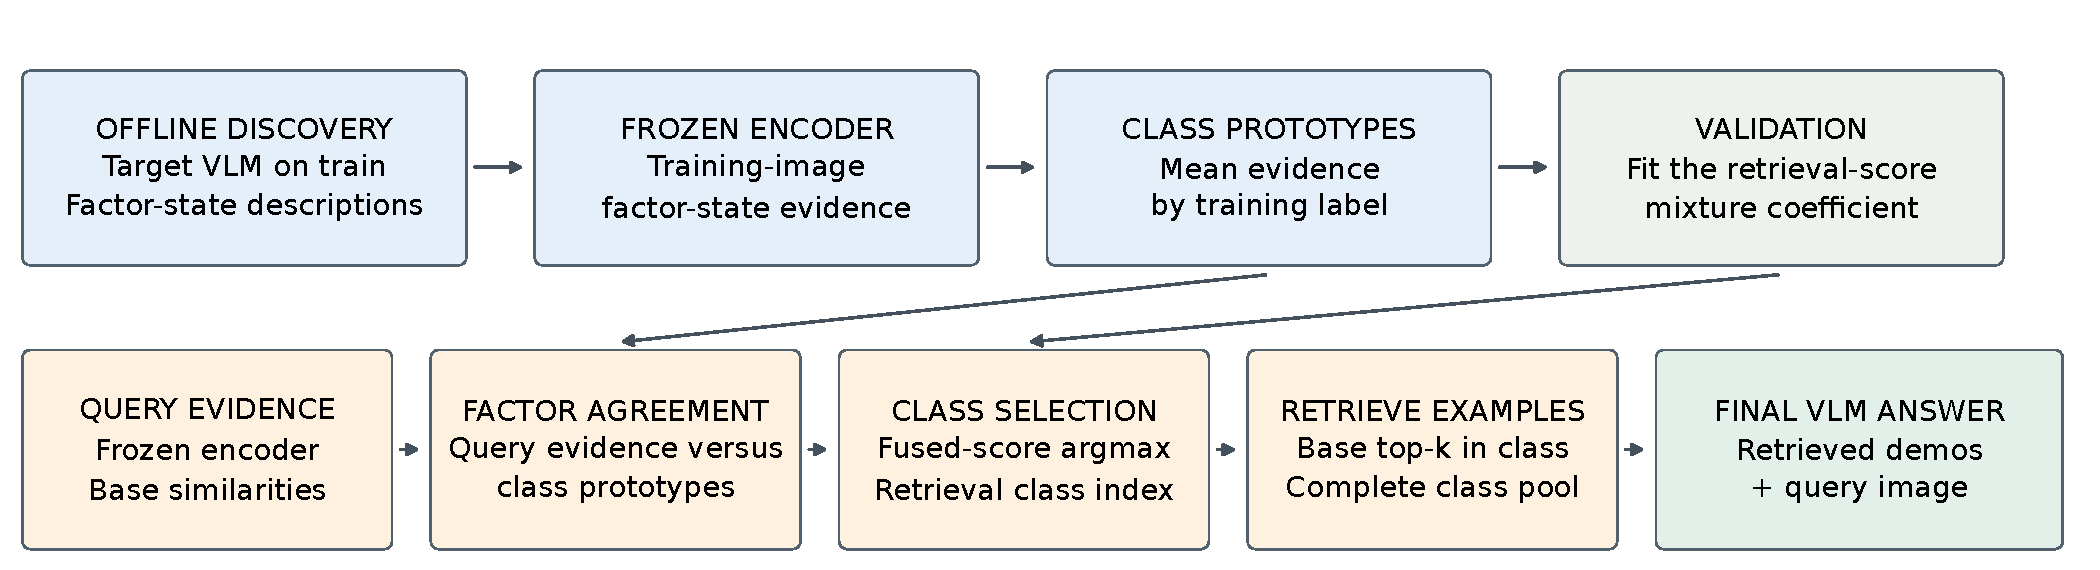
\includegraphics[width=\textwidth]{figures/pipeline.pdf}
\caption{\method separates retrieval class selection from the final VLM answer. Offline factor discovery uses the target VLM on training images. A frozen encoder measures factor states and training labels define class prototypes. At query time, class selection takes the argmax of fused retrieval scores. This class index identifies the pool for within-class retrieval. The final VLM answer is generated after the demonstrations and query enter the classification prompt.}
\label{fig:pipeline}
\end{figure*}

\section{Related Work}
\label{sec:related}
\paragraph{Visual demonstration selection.}
Flamingo performs multimodal inference using interleaved visual demonstrations~\cite{flamingo}. RICES selects examples using image similarity~\cite{rices,flamingo}, and MUIER studies textual information in multimodal retrieval~\cite{muier}. CoDR constructs a coreset, a compact subset of candidate examples, to guide demonstration selection~\cite{codr}. These methods organize context construction through similarity and the structure of the candidate pool. \method adds a representation of visual factors elicited from the target VLM and uses training-class prototypes to guide a base retriever.

\paragraph{Attribute-guided context construction.}
CIRCLES identifies visual attributes and generates counterfactual descriptions, which describe an image after changing an attribute~\cite{circles}. Image and description retrieval then supply complementary demonstrations. Our procedure uses a reusable collection of factor states to measure both queries and training classes. Their agreement guides class selection before individual examples are retrieved. This representation can accompany a single similarity ranking or the image and description rankings used by CIRCLES.

\paragraph{Language descriptions for visual recognition.}
CLIP and SigLIP 2 map images and text into comparable representations~\cite{clip,siglip2}. Classification by description uses generated visual descriptors as recognition criteria~\cite{descriptions}. Label-free concept bottleneck models use language concepts as intermediate features~\cite{lfcbm}. \method uses factor-state descriptions to construct class prototypes for demonstration retrieval. The target VLM supplies the descriptions offline. A frozen encoder measures image compatibility. Validation data determine its contribution to class selection.

\section{DecisionICL}
\label{sec:method}
Let $\train=\{(x_i,y_i)\}_{i=1}^N$ be a labeled training pool with $N$ images. Its class set $\classes$ contains $C$ classes. A separate validation set is denoted by $\valid$. Retrieval assembles an ordered sequence $D_k(q)$ of $k$ demonstrations for a query image $q$. The fixed target VLM $M$ then generates its final class answer from the resulting prompt. We use \emph{$k$-shot} to mean that exactly $k$ labeled images appear in this prompt, with $k\in\{1,2\}$. The full training pool remains available for retrieval. A base retriever $P$ assigns a similarity score $s_P(q,i)$ between query $q$ and training image $x_i$. Figure~\ref{fig:pipeline} shows how class selection determines which training class supplies the demonstrations.

\subsection{Discovering Decision Factors}
\label{sec:factors}
Offline discovery supplies the target VLM with a task-specific subset of training images and the task's class names. The instruction asks for visible properties that help distinguish the classes. Each response specifies a property through a question and descriptions of its possible states. Requests cover complementary aspects of appearance. These include shape and texture as well as pose and local visual differences. Format checks and the frozen processing protocol produce a \emph{factor bank}. This bank is retained for the target model and dataset.

Let $G$ be the number of decision factors. Factor $g$ has $S_g$ states with descriptions $\{t_{g,s}\}_{s=1}^{S_g}$. The bank is shared across queries and demonstration budgets for the same target and dataset. Each target generates its own bank, whose size follows its frozen discovery output. Qwen3-VL-4B retains 29 factors on Aircraft and 11 on CUB. The state descriptions establish common measurements for queries and training images. The supplement gives all bank sizes and construction details.

\subsection{Measuring Factor Evidence}
\label{sec:evidence}
A frozen SigLIP 2 Base patch16-224 encoder~\cite{siglip2} measures compatibility between an image and each state description. The text template is ``This image shows $\{\text{description}\}$.'' Let $\ell_{g,s}(x)$ denote the encoder's native image-text logit for state $s$ of factor $g$. We normalize these logits within each factor
\begin{equation}
 e_{g,s}(x)=\frac{\exp\ell_{g,s}(x)}{\sum_{u=1}^{S_g}\exp\ell_{g,u}(x)}.
 \label{eq:evidence}
\end{equation}
The resulting probability vector $e_g(x)$ is the image's \emph{factor evidence} for factor $g$. It expresses relative compatibility with the factor's states. We retain the encoder's native logit scale and precompute training-image evidence in batches.

For each class $c$, its class prototype for factor $g$ is the mean training-image evidence
\begin{equation}
 p_g(c)=\frac{1}{|\train_c|}\sum_{i\in\train_c}e_g(x_i),
 \qquad \train_c=\{i\mid y_i=c\}.
 \label{eq:prototype}
\end{equation}
Thus a prototype summarizes the distribution of visual states within a class. Several states can receive probability when appearances vary or a property is only partially visible.

We compare query evidence with the class prototype using Jensen-Shannon divergence, denoted by $\JSD$. This symmetric divergence measures the difference between two probability distributions and lies between zero and $\log 2$ when natural logarithms are used. Query-class agreement is
\begin{equation}
 a_g(q,c)=1-\frac{\JSD(e_g(q),p_g(c))}{\log 2},
 \label{eq:agreement}
\end{equation}
clipped to $[0,1]$ for numerical stability. Larger values indicate closer factor-state distributions. Every factor contributes one agreement score, independent of its number of states.

\subsection{Class Selection}
\label{sec:fusion}
The base retriever provides complementary evidence about image similarity. For a retriever with one ranking, its class score is the similarity of the best matching training image in that class
\begin{equation}
 b_P(q,c)=\max_{i\in\train_c}s_P(q,i).
 \label{eq:parent}
\end{equation}
RICES uses CLIP image similarity. Our classification-adapted MUIER score adds SigLIP image similarity to similarity between the query image and the candidate's class-name text. The text term is shared by all candidates in a class, so Eq.~\ref{eq:parent} combines that term with the best image match.

Base scores and factor agreements have different scales. For each query, we standardize each feature across the $C$ classes. Given a feature $h$, either $b_P$ or one of the $a_g$, we compute
\begin{equation}
 \widetilde h(q,c)=\frac{h(q,c)-\mu_h(q)}{\max(\sigma_h(q),10^{-6})},
 \label{eq:standardize}
\end{equation}
where $\mu_h(q)$ and $\sigma_h(q)$ are its mean and standard deviation over classes. We then form the combined class score
\begin{equation}
 S_{P,\alpha}(q,c)=\alpha\widetilde b_P(q,c)
 +\frac{1-\alpha}{G}\sum_{g=1}^G\widetilde a_g(q,c).
 \label{eq:fusion}
\end{equation}
The mixture coefficient $\alpha\in[0,1]$ weights the base score. The remaining weight is shared equally by the factors. Class selection returns the training-class index $c_{\mathrm{sel}}(q)=\argmax_{c\in\classes}S_{P,\alpha}(q,c)$. This argmax is evaluated directly on the retrieval scores. The class index determines which training images are eligible for the next retrieval step.

Our CIRCLES adaptation has two rankings. Original-image similarity $s_o$ compares query and training images. Composed-description similarity $s_t$ compares a generated description with training images. The target VLM generates this description by identifying an attribute and describing an image with a changed attribute. The base class score averages the strongest match from each ranking
\begin{equation}
 b_{\mathrm{C}}(q,c)=\tfrac{1}{2}\left(\max_{i\in\train_c}s_o(q,i)
 +\max_{i\in\train_c}s_t(q,i)\right).
 \label{eq:circles}
\end{equation}
This score is standardized and combined with factor agreement using the same rule as Eq.~\ref{eq:fusion}.

\subsection{Retrieving Demonstrations}
\label{sec:selection}
For RICES and MUIER, the selected class determines the candidates for the final ranking
\begin{equation}
 D_k(q)=\TopK_{i\in\train_{c_{\mathrm{sel}}(q)}}s_P(q,i).
 \label{eq:retrieval}
\end{equation}
Here $\TopK$ returns the $k$ highest-scoring distinct training examples in score order. Every training image in the selected class is eligible. For CIRCLES, the original-image ranking supplies one example and the composed-description ranking supplies one example, in that prompt order. These two rankings can return the same image.

Class selection and within-class ranking therefore use different summaries of the pool. Factor agreement aggregates evidence across a class, and the base score preserves similarity to individual training images. At $\alpha=1$, a single-ranking retriever selects the class of its first example and then retrieves within that class. At two shots, this endpoint still constrains both demonstrations to the same class.

\subsection{Validation Calibration}
\label{sec:calibration}
Each target model and dataset has an independently calibrated $\alpha$ for every shot count and base retriever. The objective is validation class-selection accuracy. This is the fraction of validation queries whose selected training class matches the validation label. We search $\{0,0.05,0.1,0.2,0.35,0.5,0.65,0.8,1\}$. Ties favor the larger $\alpha$. Stratified five-fold validation divides each class's validation images among five subsets. Each fold fits the coefficient on four subsets and evaluates class selection on the remaining subset. A final fit on the complete validation set supplies the coefficient for test retrieval.

The training pool defines prototypes and demonstration candidates throughout. Calibration is followed by freezing a \emph{retrieval plan}. This plan maps each query to its ordered demonstration identifiers. The target VLM then generates its final answer with the base method's classification prompt. Evaluation measures this generated answer. The retrieval class index remains an internal choice of demonstration pool.

\subsection{A Class-Selection Example}
\label{sec:worked}
Figure~\ref{fig:cases} follows a Challenger 600 query through retrieval and final inference. The standardized base score favors Embraer Legacy 600 by 2.466 to 2.268. The query's tail-state evidence is closer to the Challenger prototype. Tail design supplies the largest positive individual factor contribution. With all 29 factors and validation-selected $\alpha=0.20$, the fused scores become 1.196 for Challenger and 0.292 for Legacy. Their argmax selects the Challenger training pool for both demonstrations. Qwen3-VL-4B then gives the correct final answer Challenger 600. The original RICES context gives A319. The supplement supplies the full arithmetic and a failure trace.

\begin{figure*}[t]
\centering
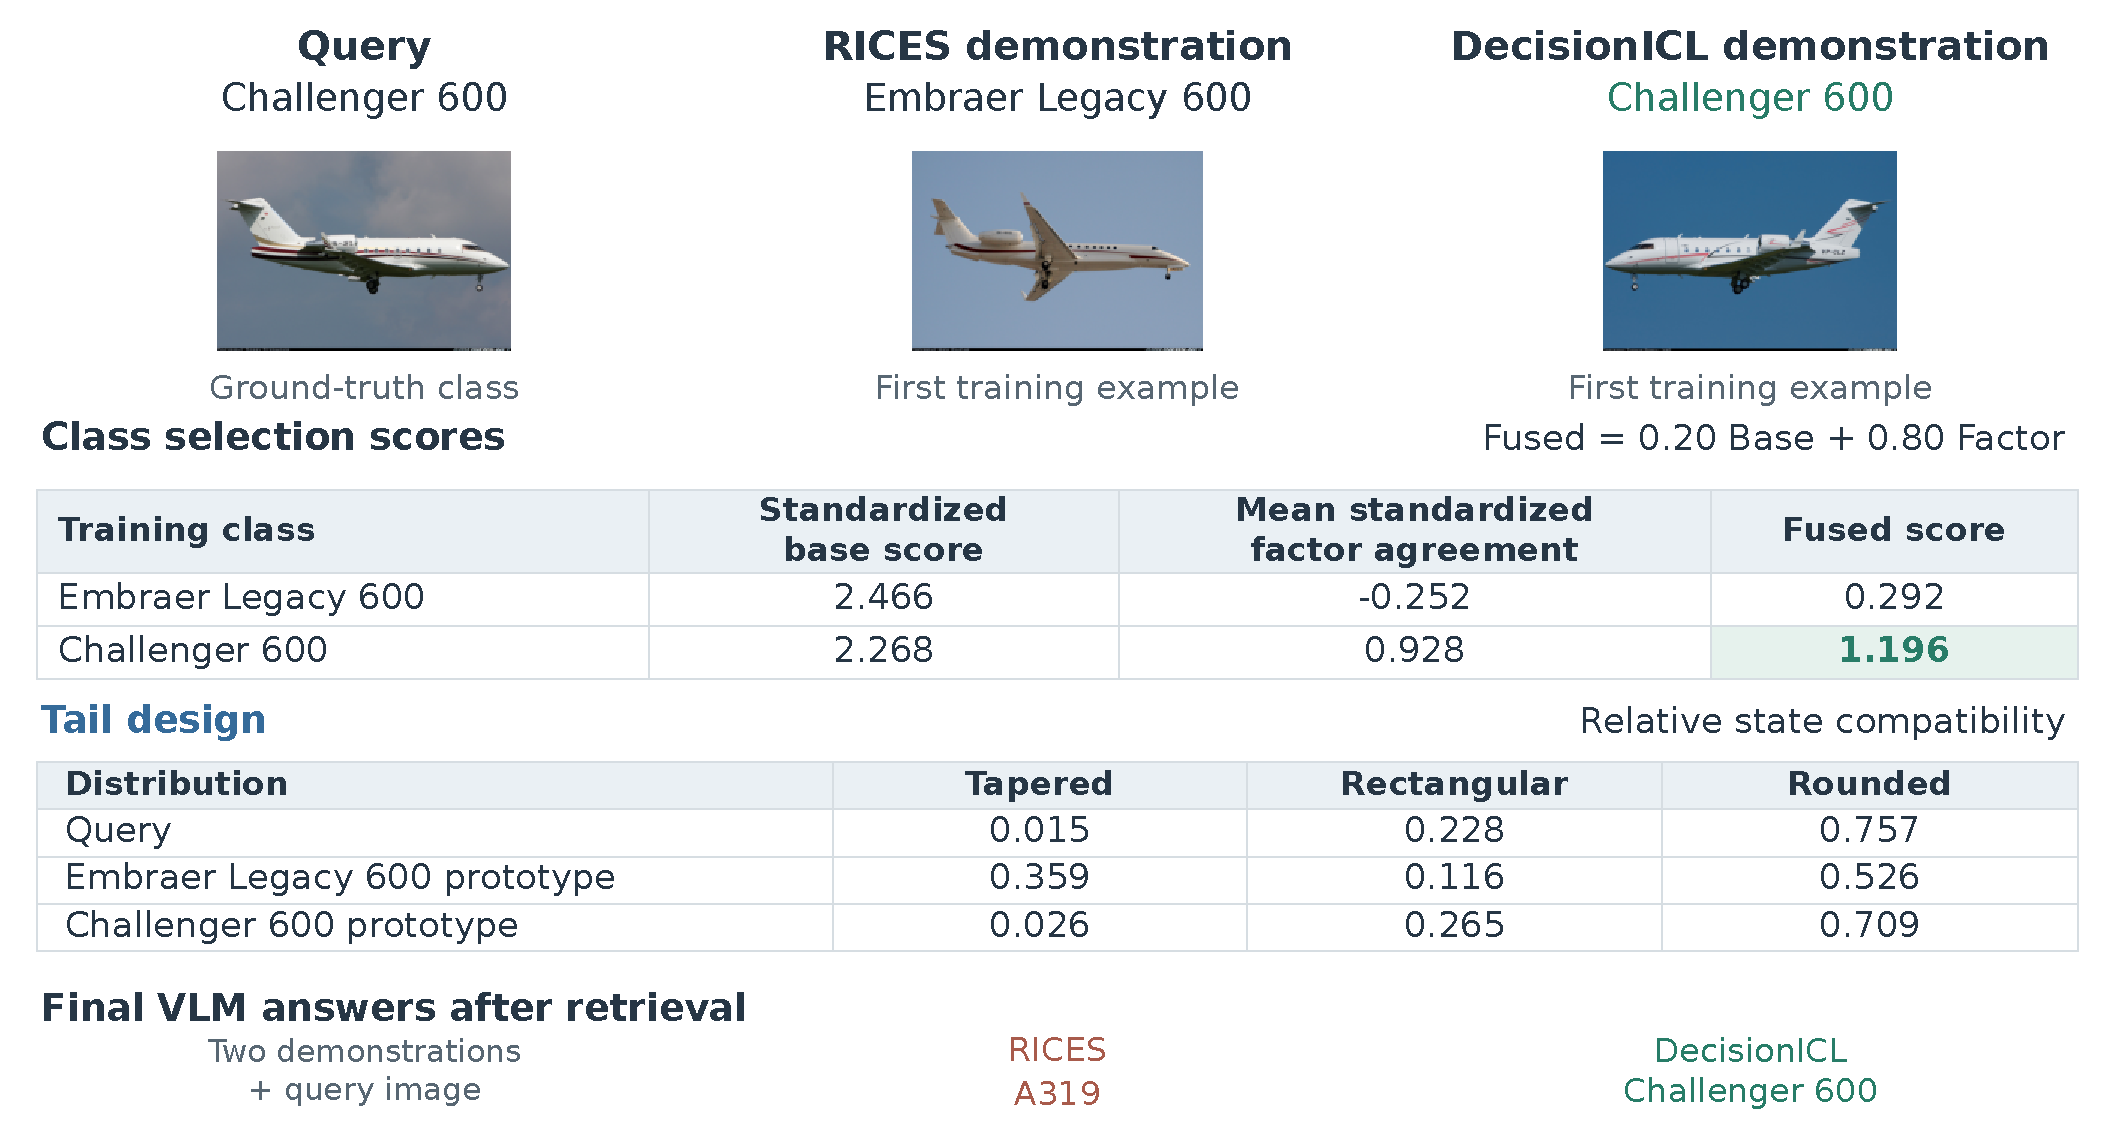
\includegraphics[width=\textwidth]{figures/retrieval_cases.pdf}
\caption{Retrieval class selection and the subsequent VLM answer for a Challenger 600 query. The top row shows the query and each method's first retrieved training example. Labels identify the images' annotated classes. The score table gives class selection by the fused-score argmax. The state table explains the tail-design contribution through measured compatibility. All 29 factors contribute to the score. The final-answer row reports VLM outputs after both demonstrations and the query enter the prompt.}
\label{fig:cases}
\end{figure*}

\section{Experiments}
\label{sec:experiments}
\subsection{Experimental Setup}
\label{sec:setup}
\paragraph{Datasets and targets.}
The datasets cover texture recognition and four fine-grained tasks. We use the Describable Textures Dataset (DTD)~\cite{dtd} for textures. The fine-grained benchmarks are FGVC-Aircraft (Aircraft)~\cite{aircraft} and CUB-200-2011 (CUB)~\cite{cub}, together with Stanford Dogs (Dogs)~\cite{dogs} and Flowers 102 (Flowers)~\cite{flowers}. DTD has 1,880 frozen test images and Aircraft has 3,333. The other test sizes are 4,794 for CUB, 8,580 for Dogs, and 6,149 for Flowers. All methods and targets share the same partitions. The supplement gives training and validation counts.

The target models are Qwen3-VL-4B-Instruct~\cite{qwen3}, Qwen2.5-VL-7B-Instruct~\cite{qwen25}, and Gemma 4 12B~\cite{gemma4}. Qwen3-VL-4B uses bfloat16 (BF16) precision. Qwen2.5-VL-7B and Gemma 4 12B use 4-bit NormalFloat (NF4) quantization with BF16 computation. Each target supplies its own factor bank and generated CIRCLES descriptions.

\paragraph{Retrieval and prompting.}
Random uniformly samples demonstrations from the training pool. The image-based methods use CLIP RICES and classification-adapted SigLIP MUIER. Their \method variants preserve the corresponding classification prompts. CIRCLES uses one image-retrieved example and one description-retrieved example. It shares the original/counterfactual prompt structure with its \method variant at the same two-example budget. Greedy decoding generates the highest-scoring next token with a limit of 512 new tokens. An inference context is the complete prompt containing demonstrations and instructions together with the query. Batches contain two contexts. The original Qwen3-VL-4B DTD one-shot block retains its fixed batch size of one. Every base-versus-\method comparison preserves its execution protocol.

\paragraph{Metrics.}
Accuracy is the fraction of test images with correct generated class names. Normalization removes surrounding whitespace and converts text to lowercase. Answers that fail to match a class name are invalid and count as errors. The supplement also reports macro accuracy, the unweighted mean of per-class accuracies, and invalid-answer counts. A \emph{rescue} is an image correct only with \method, and a \emph{harm} is an image correct only with the base method. Their count difference divided by test size gives the accuracy change. We report this change in percentage points (pp), with paired bootstrap 95\% confidence intervals (CI) from 10,000 image resamples and two-sided exact McNemar $p$ values. Five-dataset means weight each dataset equally. Differences and means are computed before rounding. The main results and component controls use the original accepted seed-42 evaluation for all three targets. In tables, +D denotes the addition of \method and $\Delta$ denotes its accuracy minus base accuracy.

\begin{table*}[t]
\caption{Final VLM accuracy from the original accepted seed-42 evaluation. Each four-row block compares RICES and classification-adapted MUIER with their respective DecisionICL variants. +MUIER identifies the SigLIP adaptation, while RICES uses CLIP. CIRCLES forms a separate two-shot group. Mean weights datasets equally. Bold marks improvement over the matching base retriever. All values are percentages.}
\label{tab:main}
\centering\small
\setlength{\tabcolsep}{3pt}
\begin{tabular}{llrrrrrr}
\toprule
$k$ & Retrieval setting & DTD & Aircraft & CUB & Dogs & Flowers 102 & Mean \\
\midrule
\multicolumn{8}{l}{\textbf{Qwen3-VL-4B-Instruct (BF16)}} \\
\addlinespace[2pt]
1 & RICES base & 76.06 & 56.62 & 74.30 & 72.74 & 92.75 & 74.49 \\
 & +MUIER & 76.28 & 61.45 & 71.01 & 76.48 & 90.96 & 75.23 \\
 & +DecisionICL & \textbf{77.55} & \textbf{65.38} & \textbf{75.39} & \textbf{74.37} & \textbf{93.15} & \textbf{77.17} \\
 & +MUIER+DecisionICL & \textbf{77.55} & \textbf{64.75} & \textbf{71.90} & \textbf{76.77} & \textbf{92.75} & \textbf{76.74} \\
\addlinespace[3pt]
2 & RICES base & 77.87 & 59.20 & 79.10 & 77.41 & 97.25 & 78.17 \\
 & +MUIER & 78.40 & 62.77 & 75.51 & 81.42 & 94.16 & 78.45 \\
 & +DecisionICL & \textbf{78.78} & \textbf{65.71} & \textbf{80.77} & \textbf{78.24} & \textbf{97.28} & \textbf{80.15} \\
 & +MUIER+DecisionICL & \textbf{79.04} & \textbf{65.26} & \textbf{76.43} & \textbf{81.56} & \textbf{96.67} & \textbf{79.79} \\
\addlinespace[3pt]
2 & CIRCLES base & 77.18 & 57.10 & 75.62 & 74.15 & 94.55 & 75.72 \\
 & +DecisionICL & \textbf{78.99} & \textbf{65.56} & \textbf{77.05} & \textbf{74.94} & \textbf{96.05} & \textbf{78.52} \\
\midrule
\multicolumn{8}{l}{\textbf{Qwen2.5-VL-7B-Instruct (NF4)}} \\
\addlinespace[2pt]
1 & RICES base & 65.05 & 51.37 & 70.34 & 68.66 & 94.41 & 69.96 \\
 & +MUIER & 66.54 & 53.62 & 67.06 & 74.50 & 91.87 & 70.72 \\
 & +DecisionICL & \textbf{66.65} & \textbf{53.59} & \textbf{72.55} & \textbf{72.53} & \textbf{94.91} & \textbf{72.04} \\
 & +MUIER+DecisionICL & \textbf{67.82} & \textbf{54.61} & \textbf{69.36} & \textbf{75.08} & \textbf{93.74} & \textbf{72.12} \\
\addlinespace[3pt]
2 & RICES base & 66.86 & 57.16 & 75.64 & 72.49 & 97.11 & 73.85 \\
 & +MUIER & 69.41 & 58.90 & 72.32 & 77.94 & 94.24 & 74.56 \\
 & +DecisionICL & \textbf{70.43} & \textbf{62.44} & \textbf{78.99} & \textbf{75.41} & \textbf{97.76} & \textbf{77.00} \\
 & +MUIER+DecisionICL & \textbf{71.17} & \textbf{61.96} & \textbf{75.53} & \textbf{78.93} & \textbf{97.35} & \textbf{76.99} \\
\addlinespace[3pt]
2 & CIRCLES base & 70.43 & 50.11 & 66.60 & 64.94 & 87.80 & 67.98 \\
 & +DecisionICL & \textbf{72.98} & \textbf{61.00} & \textbf{73.74} & \textbf{70.96} & \textbf{93.58} & \textbf{74.45} \\
\midrule
\multicolumn{8}{l}{\textbf{Gemma 4 12B (NF4)}} \\
\addlinespace[2pt]
1 & RICES base & 72.18 & 51.49 & 73.61 & 62.31 & 90.89 & 70.10 \\
 & +MUIER & 73.83 & 57.82 & 69.40 & 69.98 & 89.35 & 72.07 \\
 & +DecisionICL & \textbf{74.04} & \textbf{56.71} & \textbf{75.84} & \textbf{66.97} & \textbf{91.53} & \textbf{73.02} \\
 & +MUIER+DecisionICL & \textbf{75.59} & \textbf{59.71} & \textbf{71.84} & \textbf{70.61} & \textbf{91.58} & \textbf{73.86} \\
\addlinespace[3pt]
2 & RICES base & 73.09 & 52.03 & 74.43 & 66.83 & 94.88 & 72.25 \\
 & +MUIER & 75.11 & 59.83 & 70.61 & 74.86 & 92.34 & 74.55 \\
 & +DecisionICL & \textbf{74.57} & \textbf{59.08} & \textbf{77.47} & \textbf{71.64} & \textbf{95.56} & \textbf{75.67} \\
 & +MUIER+DecisionICL & \textbf{76.33} & \textbf{61.78} & \textbf{73.90} & \textbf{75.80} & \textbf{95.09} & \textbf{76.58} \\
\addlinespace[3pt]
2 & CIRCLES base & 71.97 & 35.01 & 64.98 & 53.08 & 86.18 & 62.24 \\
 & +DecisionICL & \textbf{75.27} & \textbf{46.14} & \textbf{72.92} & \textbf{62.05} & \textbf{92.05} & \textbf{69.69} \\
\bottomrule
\end{tabular}
\end{table*}

\subsection{Main Results}
\label{sec:mainresults}
Table~\ref{tab:main} reports all five datasets in three target-model panels. A matched setting fixes a target and dataset together with a base retriever and demonstration budget. DecisionICL has a higher accuracy point estimate in all 75 settings. Each panel uses the original accepted evaluation. The equal-setting mean gain is 2.06 pp for Qwen3-VL-4B. It is 3.11 pp for Qwen2.5-VL-7B and 3.52 pp for Gemma 4 12B. The supplement gives all per-dataset metrics and paired comparisons.

The gains extend across retrieval schemes. For Qwen3-VL-4B, mean RICES accuracy increases from 74.49\% to 77.17\% at one shot and from 78.17\% to 80.15\% at two shots. MUIER increases from 75.23\% to 76.74\% and from 78.45\% to 79.79\%, respectively. Two-shot CIRCLES increases from 75.72\% to 78.52\%. The per-dataset columns show larger benefits on Aircraft and smaller changes on Flowers 102, where two-shot RICES already exceeds 94\% for all targets.

Image-level paired analyses use the same final VLM answers as Table~\ref{tab:main}. On Qwen3-VL-4B Aircraft with two-shot RICES, DecisionICL rescues 393 images and harms 176. The gain is 6.51 pp with a 95\% CI of $[5.10,7.89]$. Intervals lie above zero in 21 of 25 Qwen3-VL-4B comparisons. The corresponding counts are 25 of 25 for Qwen2.5-VL-7B and 24 of 25 for Gemma 4 12B. The supplement gives all paired intervals and exact $p$ values.

\paragraph{Additional retrieval protocols.}
The supplementary experiments also cover a VICL task adaptation~\cite{vicl} with textual demonstrations generated from training images. At two shots, its five-dataset mean rises from 59.72\% to 69.32\% with Qwen3-VL-4B BF16. With Qwen2.5-VL-7B NF4 it rises from 63.12\% to 73.22\%. DecisionICL also improves a Prompt-SelF spatial-retrieval adaptation~\cite{promptself} using corresponding CLIP patch features. All 20 VICL comparisons and all 10 Prompt-SelF comparisons have positive accuracy differences. These are separate adapted protocols with complete single-run results in the supplement. MMICES~\cite{mmices} question-only reranking gives the RICES plans under the frozen classification protocol.

\subsection{Removing Factor Evidence}
\label{sec:gateablation}
The main procedure changes class selection and constrains demonstrations to one class. We compare the full selector with \emph{base-class selection}, which chooses the class of the first RICES example and retrieves the two highest-scoring images from that class's complete training pool. This ablation retains same-class retrieval and uses no learned parameters. Qwen3-VL-4B, its classification prompt, and the two-example budget remain fixed. We evaluate the complete DTD, Aircraft, and CUB test partitions.

\begin{table*}[t]
\caption{Removing factor evidence while retaining same-class retrieval. Base-class selection uses the first RICES example to choose a class and retrieves that class's best two examples. The last column gives \method minus base-class selection in pp with paired 95\% CIs.}
\label{tab:gate}
\centering\small
\setlength{\tabcolsep}{9pt}
\begin{tabular}{lrrrr}
\toprule
Dataset & RICES & Base-class selection & DecisionICL & $\Delta$ [95\% CI] \\
\midrule
DTD & 77.87 & 76.91 & \textbf{78.78} & +1.86 [0.80, 2.93] \\
Aircraft & 59.20 & 56.56 & \textbf{65.71} & +9.15 [7.83, 10.47] \\
CUB & 79.10 & 79.50 & \textbf{80.77} & +1.27 [0.69, 1.86] \\
\bottomrule
\end{tabular}
\end{table*}

Table~\ref{tab:gate} shows that the same-class constraint alone changes RICES accuracy by $-0.96$ pp on DTD. The change is $-2.64$ pp on Aircraft and $+0.40$ pp on CUB. DecisionICL exceeds base-class selection by 1.86 pp on DTD. Its advantages are 9.15 pp on Aircraft and 1.27 pp on CUB. All three paired CIs lie above zero. The calibrated class-selection rule improves over this parameter-free rule in the evaluated setting.

The two class-selection rules differ for 209 of 1,880 DTD queries. They differ for 1,004 of 3,333 Aircraft queries and 299 of 4,794 CUB queries. These are changes to the training class that supplies demonstrations. The counts are computed from frozen retrieval plans after evaluation. The supplement also records execution variation when ordered demonstrations coincide.

\subsection{Class Correspondence and Factor Sources}
\label{sec:controls}
We test the association between classes and factor evidence by rotating the class prototypes. A fixed one-step cyclic rotation reassigns prototypes among training classes while retaining the factor bank and image measurements. The variant receives independent validation calibration. On Qwen3-VL-4B two-shot RICES, it falls 2.07 pp below \method on DTD and 9.09 pp below it on Aircraft. On CUB, calibration selects $\alpha=1$, yielding the base-class selection accuracy of 79.50\%. The control measures the effect of class-factor correspondence where calibration retains factor evidence.

A matched-source experiment examines the descriptions used to build this evidence. \emph{Decision} discovery asks for task-discriminative factors, and \emph{Generic} discovery asks for general visual properties. Both use the same class-prototype procedure with matched training images, request budgets, and structured output format. These separately constructed banks differ from the final main-table banks. Each source receives its own calibration. For one-shot DTD, Decision minus Generic is $-0.37$ pp with RICES and $+0.53$ pp with MUIER. For Aircraft, the differences are $+1.14$ and $+0.69$ pp. The effect of the discovery instruction varies across these four settings.

A visual class-centroid control uses cosine similarity to each class's normalized mean CLIP embedding in place of factor agreement. It receives its own mixture calibration and retains within-class retrieval followed by final VLM inference. Its final VLM accuracy relative to \method is $+0.43$ pp on DTD, $-1.89$ pp on Aircraft, and $+5.05$ pp on CUB. The relative effectiveness of these class representations depends on the dataset.

A separately calibrated Generic procedure scores individual training samples directly. Across the 25 original Qwen3-VL-4B settings it is below \method in 24 settings, with a mean difference of $-1.36$ pp. This comparison changes the retrieval structure together with the factor source. The four matched-source settings above isolate the discovery instruction within a common architecture. The supplement reports both comparisons and the auxiliary protocols' Generic results.

\subsection{Calibration and Retrieval Changes}
\label{sec:calibrationanalysis}
We inspect coefficients and retrieval plans to understand how the factors enter the procedure. All 75 full-validation fits give positive weight to both base similarity and factor agreement, with $\alpha$ from 0.10 to 0.80. In 39 settings, every fold selects the same coefficient as the full-validation fit. The largest absolute difference between a fold coefficient and the full-validation coefficient is 0.15. These measurements describe calibration behavior across subsets of the available validation data.

\begin{table}[t]
\caption{Percentage of query-budget instances whose ordered demonstrations change from the base plan. RICES and MUIER pool one- and two-shot instances. CIRCLES uses two-shot instances.}
\label{tab:changes}
\centering\small
\setlength{\tabcolsep}{7pt}
\begin{tabular}{lrrr}
\toprule
Target & RICES & MUIER & CIRCLES \\
\midrule
Qwen3-VL-4B & 22.6 & 12.9 & 63.1 \\
Qwen2.5-VL-7B & 22.8 & 14.5 & 83.7 \\
Gemma 4 12B & 24.1 & 14.2 & 80.5 \\
\bottomrule
\end{tabular}
\end{table}

Table~\ref{tab:changes} reports changes in the retrieved context. DecisionICL changes 12.9\% to 24.1\% of ordered RICES and MUIER contexts across targets. CIRCLES changes more often because its two rankings can retrieve from different classes. DecisionICL uses class selection to choose one training class for both channels. The accuracy tables measure the final VLM answers generated from these contexts.

\subsection{Selected Class and Final Answer}
\label{sec:readout}
We score the selected training class against each query label and compare this readout with the final VLM answer. For Qwen3-VL-4B BF16 RICES+DecisionICL at two shots, the final VLM gains 3.59 pp over this readout on Dogs and 0.72 pp on Aircraft. It loses 0.52 pp on CUB. At one shot, the differences on CUB and Flowers 102 are $-5.90$ and $-4.02$ pp. The VLM can correct an incorrect selection or depart from a correct one. Its net effect depends on the task and demonstration budget. The supplement reports all five datasets and the paired correction counts.

\subsection{Demonstration Budget}
\label{sec:analysis}
We evaluate four, eight, and sixteen demonstrations with Qwen3-VL-4B RICES on DTD and CUB in an exploratory fixed-selector analysis. The class-selection coefficient retains its two-shot value as more examples enter the prompt. At sixteen shots, this extension is 2.23 pp below RICES on DTD and 1.75 pp below it on CUB. RICES can retrieve examples from additional classes as its budget grows, while the extension continues to retrieve within its fixed selected class. These results describe increasing context under a fixed two-shot selector. The independently calibrated comparisons in the main matrix concern one and two demonstrations.

\section{Discussion}
\label{sec:discussion}
\method connects two decisions in context construction. Factor agreement and base similarity select a class, and the base ranking chooses demonstrations within it. The worked example makes this score-to-context mapping explicit. The Qwen3-VL-4B component ablation shows that the calibrated selector exceeds choosing the first RICES example's class on three complete test partitions.

The evidence describes image compatibility with target-generated text. Its effectiveness depends on both that text and the frozen encoder, as reflected by the mixed source and visual-centroid results. Offline discovery and training-image measurements are reused across queries. Query measurement and class agreement add work during retrieval. The final-answer analysis separates selection quality from subsequent VLM behavior. A high-margin failure trace shows how factor evidence can redirect retrieval to an incorrect class. Selecting several plausible classes is a natural extension for larger budgets.

\section{Conclusion}
We presented \method for visual demonstration selection using factors elicited from the target VLM. A frozen encoder measures factor states. Labeled training images define class prototypes. Validation calibration combines factor agreement with base similarity for class selection. The selected training class supplies demonstrations through complete within-class retrieval. The target VLM then generates the final query answer. Accuracy differences are positive in all 75 matched settings across five datasets and three target models. The Qwen3-VL-4B two-shot RICES component comparison further supports the calibrated class-selection rule on three datasets. These findings establish an empirical benefit for the evaluated retrieval procedure at small demonstration budgets.

{\small
\bibliographystyle{ieeenat_fullname}
\bibliography{references}
}
\end{document}
